%LaTeX source for the ACL 2011 Demo submission for the Topical Guide project
%TODO: Read topic naming papers

%In case we change the name of the build script, we define a macro for it:
\newcommand{\buildscript}{backend.py}
\newcommand{\tool}{Topical Guide}
\newcommand{\projecturl}{http://nlp.cs.byu.edu/topicalguide}

\documentclass[11pt]{article}
\usepackage{acl-hlt2011}
\usepackage{times}
\usepackage{latexsym}
\usepackage{amsmath}
\usepackage{multirow}
\usepackage{url}
\usepackage{graphicx}
\usepackage{listings}	
\DeclareMathOperator*{\argmax}{arg\,max}
\setlength\titlebox{6.5cm}    % Expanding the titlebox

\title{Increased Comprehension of Topic Models and Corpora Using the \tool}
\author{Josh Hansen, Matthew J. Gardner, Jeff Lund, Dan Walker, Eric Ringger, \and Kevin Seppi\\
Department of Computer Science\\
Brigham Young University\\
\tt \{mjg82,jlutes,joshhansen\}@byu.edu, \{jefflund,danwalkeriv\}@gmail.com\\
\tt \{ringger,kseppi\}@cs.byu.edu}

\begin{document}
\maketitle

\begin{abstract}
Though topic models reduce dimensionality, their output is just as large as the training corpus.
Thus, humans' ability to manually assess model quality is limited. As digitization of historic texts
proceeds at breakneck pace, institutions correspondingly find an increased need for tools such as
topic models to make these texts usable. In response to these twin needs, we present the \tool,
an open-source\footnote{Licensed under the terms of the
Affero General Public License, version 3.} web application for interactive, topic-centric
exploration and visualization of topic model output.
We explain why such a tool is warranted, what it is capable of, and
how to use it to explore the corpus or topic model of your choice.
\end{abstract}

\section{Introduction}
Since its introduction, LDA-based topic modeling \cite{blei_latent_2003} has
become standard fare for those wishing to automatically distill large text
collections into something more immediately useful to humans and computers
alike. The usefulness of this sort of dimensionality reduction is widely
acknowledged, and topic models continue to be extended into exciting new
territory.
\cite{wang_continuous_2008,mimno_polylingual_2009,boyd-graber_holistic_2010,brody_unsupervised_2010,he_detecting_2009,yao_efficient_2009}
However, these models output a topic assignment per token, resulting in an
output that is a corpus unto itself. Though the range of possible values is
substantially reduced, output size remains on the same order as input size.
Notwithstanding, papers introducing new topic models often lean heavily on the
hope that displaying a few hand-picked topics will convince others of the
model's effectiveness. But the very vastness of topic model output renders this
sort of presentation unconvincing. Unfortunately, tools for deep understanding
of topic model output have thus far been lacking.

Simultaneously, massive digitization efforts by libraries and other institutions
are generating gargantuan quantities of electronic text, increasing demand for tools such as
topic models. Because of their ability to characterize the contents of
corpora, topic models seem to hold great promise for archival
institutions wishing to make their newly-digitized collections accessible to
researchers and the public. However, readily available tools for exploration of 
document collections in terms of topic models have been either unsatisfactory
or nonexistent.

We present the \tool, an open-source web application for interactive,
topic-aware exploration and visualization of both document collections and the
topic models inferred on them. Further information on the project, including
source code access and a live demonstration server, can be found
at \texttt{\projecturl}.
%TODO Introduce SOTU dataset

\begin{figure*}[t]
 \centering
 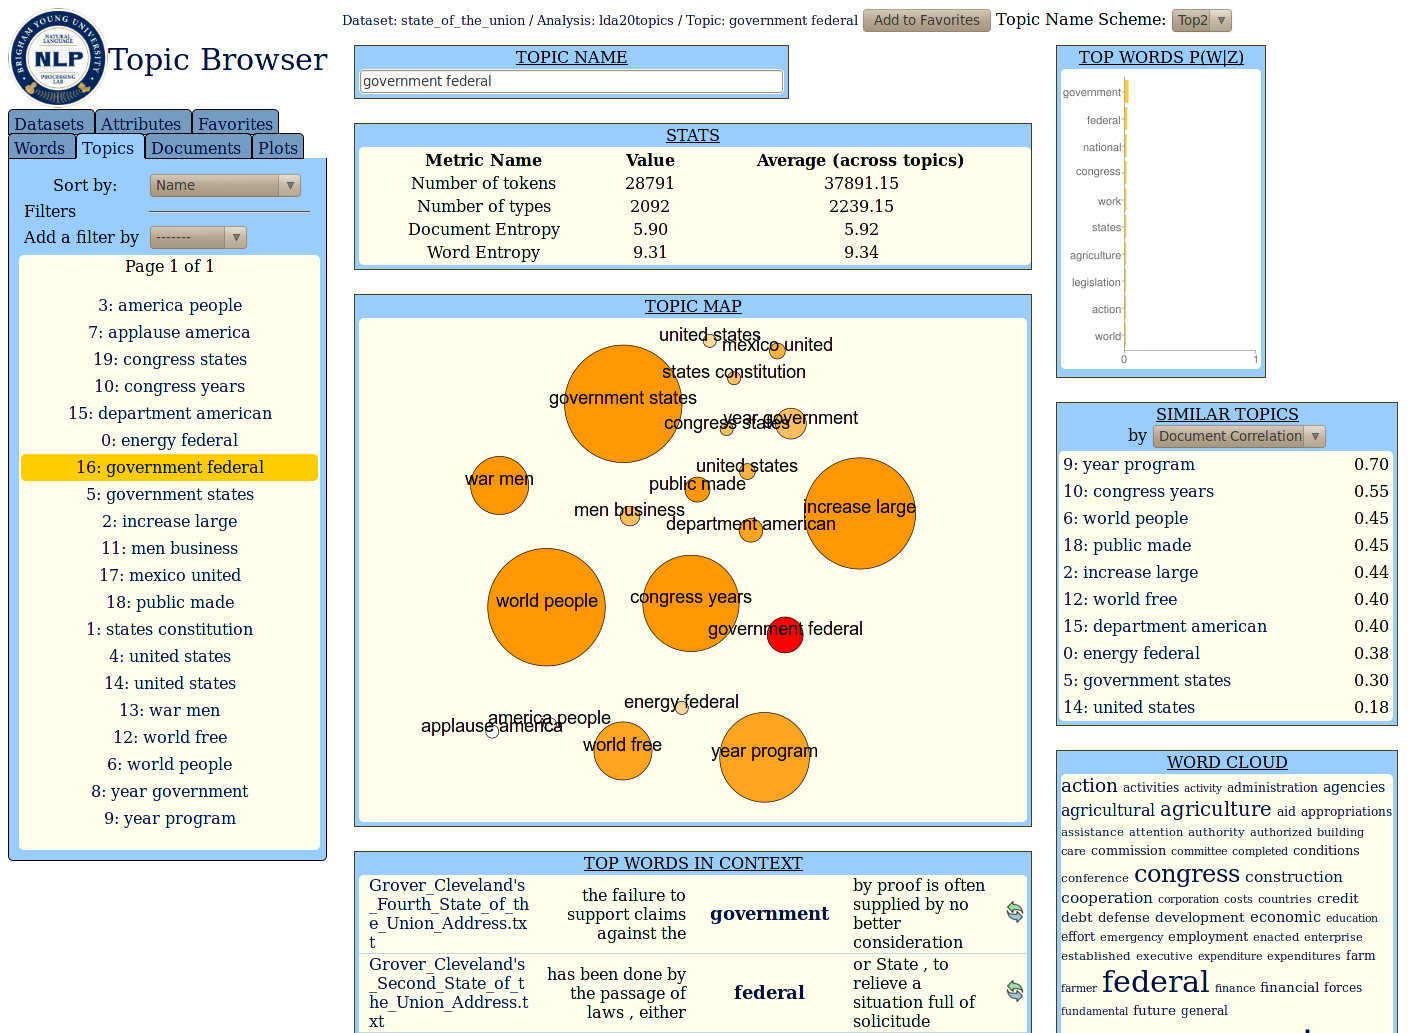
\includegraphics[width=400px,keepaspectratio=true]{./topic_page_take2.png}
 % topic_page_huge_cropped.png: 1394x1027 pixel, 96dpi, 36.88x27.17 cm, bb=0 0 1045 770
 \caption{The topic page}
 \label{fig:topic_page}
\end{figure*}

%TODO Segue

\section{Browsing}%TODO Talk about more features
The \tool{} object model and user interface include notions of
\textit{datasets} and \textit{analyses}.
A dataset is a set of documents --- a corpus. An analysis is associated with one
dataset and constitutes the set of topics and token-level topic assignments for
all of the documents in that dataset.

All entities explicitly modeled by a basic topic model --- topics, documents, and
words --- are first-class citizens in the \tool, meaning that the user
interface provides specific views for each of these entity types. For example, a
view of the ``government federal'' topic is rendered in Figure \ref{fig:topic_page}.
It displays statistics about the topic (``STATS''); chart, word-cloud, and
key-word-in-context representations of top words (``TOP WORDS $P(W|Z)$''/
``WORD CLOUD''/``TOP WORDS IN CONTEXT''), and both textual and graphical
representations of similar topics (``SIMILAR TOPICS''/``TOPIC MAP'').

Intuitive hyperlinks make this a true \textit{browsing} tool. Click on the
``government states'' node in the topic map and be sent to its topic view to see
how presidents have discussed state government. Click on ``federal'' in the word
cloud to see the word view, which shows top topics and documents in which the
word occurs. Or click on ``Grover\_\allowbreak{}Cleveland's\_\allowbreak{}Fourth\_\allowbreak{}State\_\allowbreak{}of\_\allowbreak{}the\_\allowbreak{}Union\_\allowbreak{}Address.txt''
to see President Cleveland's message with words belonging to the ``government federal''
topic highlighted.\footnote{For a more complete discussion
of browsing features see \cite{gardner_browser_2010}.}%TODO Replace with actual discussion
%TODO Make words in the doc view link
%TODO Show words in context in the word view

\subsection{Metrics}
Topic-centric document exploration is enhanced by means of \textit{metrics}.
Metrics are functions that give users additional insight into the nature of
topics or documents. They can be either unary or binary,
here called \textit{pairwise}.\footnote{Pairwise metrics do not necessarily
constitute ``metrics'' in the formal sense. We leave it to implementers to
determine whether to satisfy the triangle inequality, etc.} Topic metrics range
from simple metrics, such as the number of word tokens and types labeled with
the topic, to more complicated metrics such as dispersion across
documents, prevailing sentiment, or the semantic coherence of its words [10]. Pairwise topic metrics%TODO: Cite
include Pearson correlation on documents and on words. These are used to automatically
display a list of similar topics.

Similar to topic metrics, one can also compute document metrics. Beyond simple metrics like to-
ken count in the document, these include things such as the entropy of the topic distribution of
the document [8]. And as with topics, we make use of pairwise document metrics such as topic%TODO: Cite
correlation [3] to show similar documents.%TODO: Cite

\subsection{Charts}

\begin{figure*}[t]
 \centering
 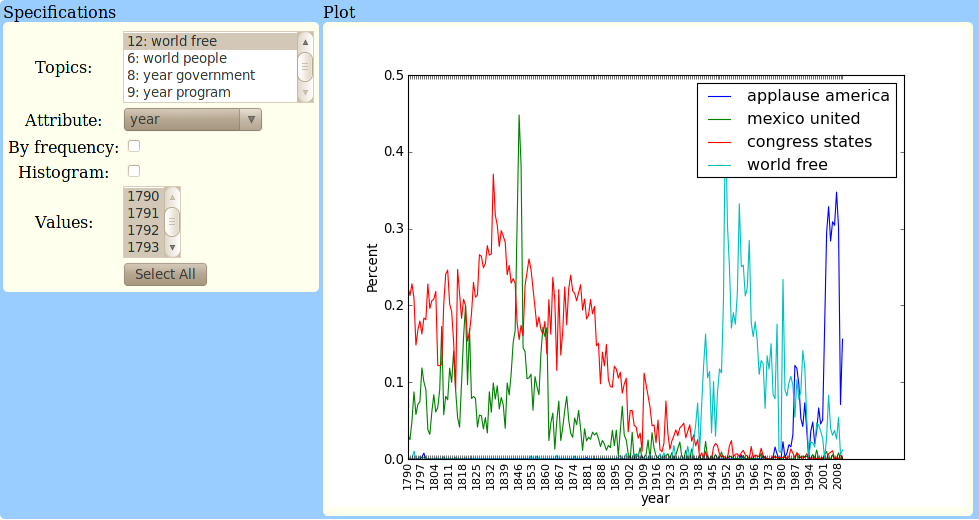
\includegraphics[height=200px,keepaspectratio=true]{./topics_vs_years.png}
 % topics_vs_years.png: 979x520 pixel, 96dpi, 25.90x13.76 cm, bb=0 0 734 390
 \label{fig:chart}
 \caption{Selected topics over time as a percentage of overall tokens.}
\end{figure*}
%TODO: Cite PNAS2005, ToT

\subsection{Topic ``Maps"}
With topic-to-topic relationships described by means of pairwise topic metrics,
graph-based visualization of the topic space becomes straightforward. In our
current implementation, we construct a topic graph $G = (N, E)$ as follows:
$N$ is a set of $|T|$ nodes such that
\[\forall_{t\in T} weight(N_{t}) = \tau_{1}(t)\]
and
\[\forall_{t\in T} color(N_{t}) \sim \tau_{2}(t)\]
where $\tau_1$ and $\tau_2$ are topic metrics (potentially the same). $E$ is
constructed as a set of $|T|^2$ edges such that
  \[\forall_{(t,u)\in T\times T, t\neq u} weight(E_{t,u}) = \pi(t,u)\]
where $\pi$ is a pairwise topic metric.

We use the Gephi Toolkit\footnote{http://www.gephi.org} to generate such graphs
and render them as images, employing the \texttt{ForceAtlas} force-directed
layout algorithm to arrange the nodes so that, generally speaking, nodes joined
by edges of higher weight are closer together, and nodes joined by edges of
lower weight are further apart.

%TODO Callback

\subsection{Topic Name Schemes}
As LDA does not assign names to the topics it generates, automatic generation of
topic names is of interest to researchers wishing to make topic models
human-usable. Research in this area is ongoing \cite{Mei2007,Lau2010}. In order to
facilitate investigations in this area, we equipped the \tool{} with a
fully pluggable topic naming system. Any number of topic name schemes can be
used to produce names for all topics in an analysis. Within the user interface
users can select a name scheme, which is then reflected throughout the
interface. By default we use a concatenation of the two
words with the highest probability for a given topic $z$, but any number of
alternative schemes can be imagined and implemented. (MAYBE SHOW TF-ITF?)

\section{Data Import Backend}
\begin{figure*}[t]
 \centering
 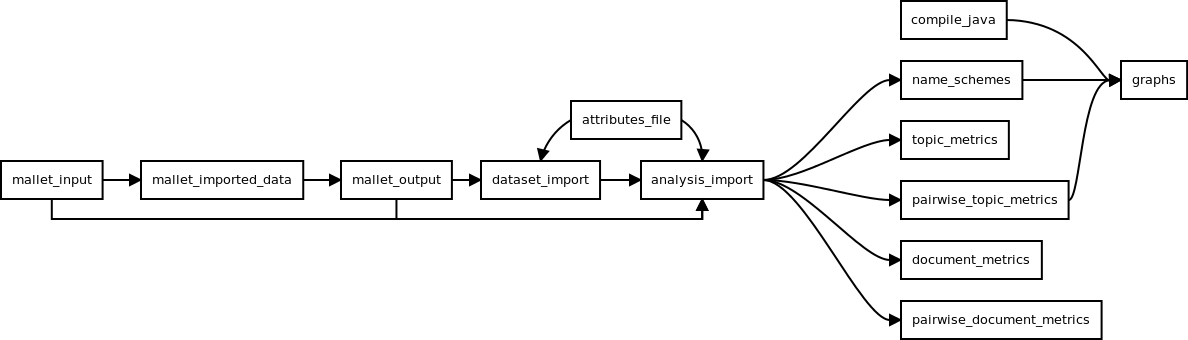
\includegraphics[width=400px,keepaspectratio=true]{./build_flowchart.png}
 % build_deps.png: 1188x340 pixel, 72dpi, 41.91x11.99 cm, bb=0 0 1188 340
 \caption{The data import pipeline. Arrows indicate that the source is prerequisite for the target.}
 \label{fig:build_flowchart}
\end{figure*}

Automatically turning a raw document collection into an interactive browsing
experience requires extensive preprocessing. Documents must be converted into a
representation accepted by the topic model learner. Topics must then be inferred
and model output indexed. Additionally, metrics must be computed, topic names
generated, and graphs rendered before they become accessible via the user
interface. Unsurprisingly, the dependencies in the import process form a directed acyclic graph, represented in Figure \ref{fig:build_flowchart}. To
improve the efficiency and usability of the data import pipeline we built a
command-line frontend based on the \texttt{doit} task automation tool.\footnote{http://doit.sourceforge.net/}

The main data import script is \texttt{\buildscript}. Some example invocations:
\begin{itemize}
 \item \texttt{\buildscript}: Builds all targets
 \item \texttt{\buildscript} list/: Lists the available top-level tasks (sub-tasks are not displayed)
 \item \texttt{\buildscript} clean -c mallet/: Cleans the Mallet files
\end{itemize}

% Useful commands:
%  \buildscript{} list #Lists the available top-level tasks (sub-tasks are not displayed)
%  \buildscript{} #Builds everything!
%  \buildscript{} clean -c mallet #Cleans the mallet files
%  \buildscript{} metrics #Computes all metrics
%  \buildscript{} topic_metrics #Computes just the topic metrics
%  \buildscript{} topic_metrics:document_entropy #Computes just the document entropy topic metric
%  \buildscript{} clean topic_metrics:document_entropy #Cleans just the document entropy topic metric

\subsection{Adding Support For Your Dataset}
Python module \texttt{build} contains dataset-specific import scripts.
Generally, a sub-module contains the scripts for a particular dataset. The
scripts for the default State of the Union Addresses dataset, for example,
reside in \texttt{build.state\_\allowbreak{}of\_\allowbreak{}the\_\allowbreak{}union}. The main build file for the dataset
is \texttt{build/\allowbreak{}state\_\allowbreak{}of\_\allowbreak{}the\_\allowbreak{}union/\allowbreak{}state\_\allowbreak{}of\_\allowbreak{}the\_\allowbreak{}union.py}. This file is
referenced within the root \texttt{\buildscript} build script by setting the
\texttt{build} variable:
\texttt{build = "state\_\allowbreak{}of\_\allowbreak{}the\_\allowbreak{}union/\allowbreak{}state\_\allowbreak{}of\_\allowbreak{}the\_\allowbreak{}union"}

A dataset-specific build must do four things:
\begin{enumerate}
\item Define \texttt{dataset\_name}.
    \newline Example: \texttt{dataset\_name='state\_of\_the\_union'}
  \item Define \texttt{dataset\_description}.
    \newline Example: \texttt{dataset\_description='State of the Union Addresses'}
  \item Ensure that all documents in the dataset are located in a single directory.
    This can be done by pointing to an existing directory (default is \texttt{dataset\_dir+'/files'}, or by overriding the
    \texttt{extract\_data} task and populating the directory on-the-fly.
  \item Provide a document metadata file in JSON format. Again, this can be done
    either by pointing to an existing file (\texttt{attributes\_\allowbreak{}file=\allowbreak{}dataset\_\allowbreak{}dir\allowbreak{}+\allowbreak{}'/attributes\allowbreak{}.json'}), or by defining a task that builds the \texttt{attributes.json} target.
\end{enumerate}

Once \texttt{build} inside of \texttt{\buildscript} has been set to point to
the dataset-specific build, \texttt{\buildscript} can be invoked to begin the
import process.

\section{Conclusion}
In this paper we introduced the \tool{} as a tool for exploration of
topic model output. This serves to improve understanding of both topic models
and text corpora. We briefly described some of the general features of the tool
and proceeded to detail the use of metrics and graphs. We then explained how
new datasets can easily be imported into the tool.

% At a minimum, the dataset-specific build file should contain the following:
% \begin{itemize}
%  \item Declaration of \verb/dataset_name/ variable.
%    \newline Example: \verb/dataset_name = "state_of_the_union"/.
%  \item Declaration of \verb/dataset_description/ variable.
%    \newline Example: \texttt{dataset_description = "State of the Union Addresses 1790-2010"}.
%  \item Definition of \verb/copy_and_transform_dataset/ \verb/doit/ task.
% Example:
% 
% \begin{figure*}
%  \centering
%   \begin{lstlisting}[numbers=left,language=Python]
% chron_list_filename = 'chronological_list.wiki'
% addresses_filename = 'state_of_the_union_addresses.txt'
% dataset_name = 'state_of_the_union'
% dataset_description = 'State of the Union Addresses 1790-2010'
% 
% def task_attributes_file():
%     task = dict()
%     task['targets'] = [attributes_file]
%     task['actions'] = [(generate_attributes_file,
%          [dataset_dir+'/'+chron_list_filename,
%           attributes_file])]
%     task['clean'] = ['rm -f '+attributes_file]
%     return task
% 
% def task_extract_data():
%     task = dict()
%     task['targets'] = files_dir
%     task['actions'] = [(extract_state_of_the_union,
%          [dataset_dir+'/'+chron_list_filename,
%           dataset_dir+'/'+addresses_filename,
%           files_dir])]
%     task['clean'] = ['rm -rf '+files_dir]
%     task['uptodate'] = [os.path.exists(files_dir)]
%     return task
% \end{lstlisting}
% \caption{The data extraction task for the State of the Union dataset. }
% \label{fig:extract_data}
% \end{figure*}
% 
% \end{itemize}

\bibliographystyle{acl}
\bibliography{acl2011demo.bib}
\end{document}

